\documentclass{article}
\usepackage{lmodern}
\usepackage{upquote}
\usepackage{cite}
\usepackage{tikz}
\usepackage[hidelinks, pdfusetitle]{hyperref}

\usetikzlibrary{positioning}

\newcommand{\pytvversion}{0.5.6}

\title{PyTV: Python Templated Verilog}
\author{Wuqiong Zhao%
  \thanks{The author was with Southeast University, Nanjing, China,
  and is now with the University of California San Diego, La Jolla, CA, USA.
  e-mail: \texttt{me@wqzhao.org}.}}

\begin{document}

\maketitle

\begin{abstract}
  PyTV (Python Templated Verilog)%
  \footnote{This is the documentation to PyTV version \texttt{\pytvversion{}}.
  Digital version of this document is available at \url{https://go.wqzhao.org/pytv-docs}.}
  is a Rust library and binary tool that extends Verilog with Python templating.
  Utilizing the flexibility of Python,
  PyTV allows users to write Verilog code with Python syntax and features
  including if statements, for loops, function definitions, etc.
  Moreover, PyTV supports instantiation of modules with complex parameters,
  and enables hierarchy extraction.
\end{abstract}

\tableofcontents

\section{Introduction}\label{sec:introduction}
% Templated languages
One method of auto generation of parameterized hardware relies on templated languages.
AHDW \cite{zhao2023automatic} is a language building upon Verilog with custom syntax for parameterized hardware.
% PyTV's advantage

Different from other domain-specific languages (DSLs) for hardware generation,
PyTV provides users with more control over the hardware architecture and implementation details.

% PyTV project information
PyTV is open-source at \url{https://github.com/autohdw/pytv}
and is distributed under the GPL-3.0 license.
The Rust crate is available at \url{https://crates.io/crates/pytv}.


\section{Installation}\label{sec:installation}
\subsection{Installation as a Rust Library}
Similar to other library crates, PyTV can be installed as a Rust library by adding the following line to the \texttt{Cargo.toml} file of your project:
\begin{verbatim}
[dependencies]
pytv = "0.5.6"
\end{verbatim}
The version number can be replaced with the desired version of PyTV.
The library can then be imported into your Rust code by adding the following line:
\begin{verbatim}
extern crate pytv;
\end{verbatim}

You can also install PyTV using the \texttt{cargo} command:
\begin{verbatim}
cargo install pytv
\end{verbatim}

\subsection{Installation as a Binary Tool}
PyTV can also be installed as a binary tool by running the following command:
\begin{verbatim}
cargo install pytv
\end{verbatim}

You can also build the binary tool from source by running the following command:
\begin{verbatim}
cargo build --release
\end{verbatim}


\section{Architecture}\label{sec:architecture}
The architecture (generation process) of PyTV is illustrated in Figure~\ref{fig:architecture}.

\begin{figure}[htbp]
  \centering
  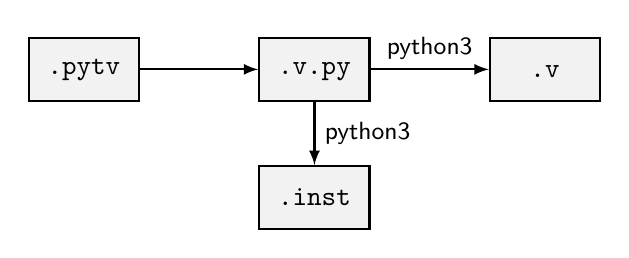
\begin{tikzpicture}[
    , thick
    , font = \sffamily
    , n/.style = {
      , draw
      , fill = gray!10
      , minimum width = 14mm
      , minimum height = 8mm
      , font = \ttfamily
      , text height = 1.3ex
    }
    , node distance = 8mm and 15mm
  ]
    \node (pytv) [n] {.pytv};
    \node (v-py) [n, right = of pytv] {.v.py};
    \node (v) [n, right = of v-py] {.v};
    \node (inst) [n, below = of v-py] {.inst};
    \draw [-latex] (pytv) -- (v-py);
    \draw [-latex] (v-py) -- (v) node [midway, above] {\small python3};
    \draw [-latex] (v-py) -- (inst) node [midway, right] {\small python3};
  \end{tikzpicture}
  \caption{Architecture of PyTV.}
  \label{fig:architecture}
\end{figure}


\section{Syntax Specifications}\label{sec:syntax}
\subsection{Basics: Python Line and Verilog Line}

\subsection{Indentation}

\subsection{Instantiation}


\section{Usage}\label{sec:usage}
\subsection{Rust Library Usage}

\textbf{Customization of the magic comment string.}

\subsection{Binary Tool Usage}


\section{Limitations}\label{sec:limitations}
\textbf{Important:}
PyTV is designed for research and prototyping purposes,
and is not intended for production use.


\section{Further Readings}\label{sec:ads}
Hardware generation using software programming languages is interesting to explore.
AHDW \cite{zhao2023automatic} is a previous attempt of implementation.
A high-level synthesis (HLS) library for Vitis HLS (in C++), FLAMES,
is proposed in \cite{zhao2024flexible}.

% auto generator of LEADS


\section*{Acknowledgments}
\addcontentsline{toc}{section}{Acknowledgments}
The author would also like to thank \textit{GitHub Copilot}
for providing code suggestions during the development of this project,
as well as the composition of this document.


\bibliographystyle{IEEEtran}
\phantomsection
\addcontentsline{toc}{section}{References}
\bgroup
\small
\bibliography{IEEEabrv, ref}
\egroup

\end{document}
